\section{Comparaison avec la photo avec effet
poster}\label{comparaison-avec-la-photo-avec-effet-poster}

\begin{figure}[htbp]
\centering
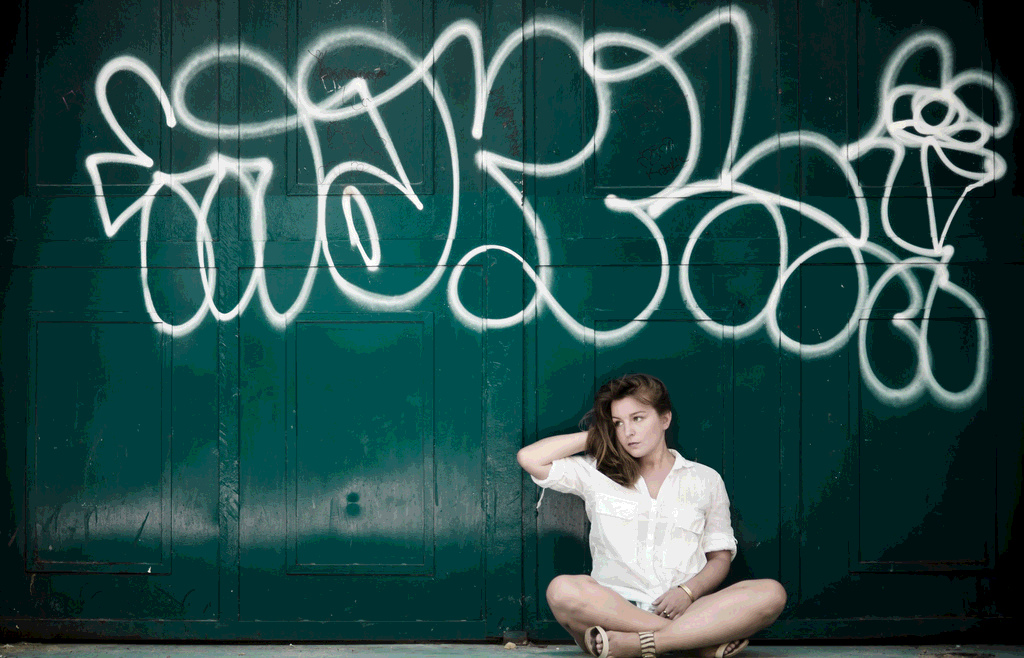
\includegraphics{../../photos/poster.jpg}
\caption{Photo poster}
\end{figure}

\begin{table}[htbp]
\centering
\begin{tabular}{llr}
\bfseries Formes &
\bfseries Bhattacharyya (\%)%
\DTLforeach*[\DTLiseq{\fichier}{photos/poster.jpg}]{valeurs}{%
\fichier=Fichier, \formes=Formes,\bhatta=Bhattacharyya, \hue=Hue, \saturation=Saturation, \value=Value}{%
\\
\formes & \bhatta}
\end{tabular}
\end{table}


La comparaison de cette image nous donne une différence de $16.35 \%$ pour la
colorimétrie avec la distance de Bhattacharyya et de $16.79 \%$ pour les formes
après application du filtre de Sobel. Ce sont des pourcentages similaires,
cependant selon nos critères, la différence colorimétrique est trop élevée pour
dire que les images se ressemblent. Cependant pour la différence de formes via
l'application du filtre de Sobel, le pourcentage est suffisamment faible pour
considérer que les images se ressemblent d'un point de vue des formes. \\
À l'\oe il nu, on peut observer que les ombres sont vraiment délimités sur la
photo poster, ce qui explique les $16 \%$ de différence trouvés après
application du filtre de Sobel.
